\documentclass[14pt]{beamer}
\title[JPL:Java:02]{JPL :: Modular Programming - 1}
\author[TS]{TalentSprint}
\institute[L\&D]{Licensed To Skill}
\date{Version 1.0.4}
\usefonttheme{serif}
\usecolortheme{orchid}
\usepackage{bookman}
\usepackage{hyperref}
\usepackage[T1]{fontenc}
\usepackage{graphicx}
\usepackage{listings}
\graphicspath{{../../Images/}}
\beamertemplateballitem
\usebackgroundtemplate{
\includegraphics[width=\paperwidth]{TS-XP-Logo.jpg}}
\lstset{language=Java,numbers=left, numberstyle=\tiny, basicstyle=\footnotesize, numbersep=10pt, showstringspaces=false, breaklines=true,keepspaces=true, columns=flexible}
\begin{document}

\begin{frame}
  \titlepage
\end{frame}

\begin{frame}{Learning Objectives}
By the end of this presentation, you are able to:
  \begin{itemize}
  \item Write programs to problems by decomposing functionality into methods and using the methods
  \item Write computationally efficient programs
  \item Create meaningful functional decomposition systematically
  \item Develop and test your programs progressively
  \end{itemize}
\end{frame}

\begin{frame}{Modular Programming - 1}
 \begin{figure}[H]
  \begin{minipage}{5cm}
   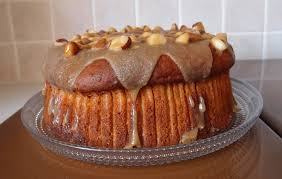
\includegraphics[scale=.4]{modular-programming-cake1.png}
  \end{minipage}
  \quad
  \begin{minipage}{5cm}
   
\includegraphics[scale=.4]{modular-programming-cake2.png}
  \end{minipage}
 \end{figure}

 \begin{figure}[H]
  \begin{center}
   
\includegraphics[scale=.4]{modular-programming-cake3.png}
  \end{center}

 \end{figure}

\end{frame}

\begin{frame}[fragile]{Modular Programming - 1}
\begin{minipage}{7.5cm}
\begin{lstlisting}[numbers=none]
public static void main(String[] args) {
  
    Reading responsibility ============>

    Arithmetic responsibility ==========>

    Perfect Number responsibility ======>
    
    Prime responsibility ==============>

    Factorial responsibility ===========>
}
\end{lstlisting}
\end{minipage}
\quad
\begin{minipage}{2cm}
 \colorbox{cyan}{Why?}
\end{minipage}
\end{frame}

\begin{frame}[fragile]{Modular Programming - 1}
Finding Factorial of a given number...
 \begin{minipage}{5.5cm}
  \begin{lstlisting}[numbers=none]
... void main(String[] args) {
    int i, n = 5; 
    int factorial = 1;
    for (i = 1; i <= n; i++) {
        factorial = factorial * i;
    }
    System.out.print(factorial);
}
  \end{lstlisting}
 \end{minipage}
\quad
\begin{minipage}{4cm}
\begin{table}
 \tiny
 Before entering loop n = 5, factorial = 1
 \begin{tabular}{|p{1cm} | p{.5cm} | p{1.2cm} |}
 \hline
  \textbf{factorial} & \textbf{i} & \textbf{condition} \\ \hline
  1 & 1 & 1 <= 5 \\ \hline
  1 & 2 & 2 <= 5 \\ \hline
  2 & 3 & 3 <= 5 \\ \hline
  6 & 4 & 4 <= 5 \\ \hline
  24 & 5 & 5 <= 5 \\ \hline
  120 & 6 & \color{red}{6 <= 5} \\ \hline
 \end{tabular}
\end{table}
\end{minipage}
\end{frame}



\begin{frame}{Modular Programming - 1}
\small
 Let us now learn more about methods in Java...
 \begin{itemize}
  \item A method is a set of instructions implemented in order to perform a specific task.
  \item All methods in Java must be defined inside some class. Main method is also part of a class.
  \item Methods are identified by their signature.
  \item Signature contains method name and the parameters it takes. Each method in Java should have four parts.
  \begin{itemize}
   \item Return-type
   \item Method-name
   \item Parameters
   \item Method body
  \end{itemize}

 \end{itemize}
\end{frame}

\begin{frame}[fragile]{Modular Programming - 1}
 Writing Methods
 \begin{block}{Syntax}
  \begin{lstlisting}[numbers=none]
<return-type> <method-name>(<parameters>) {
    statement(s);
}
  \end{lstlisting}
 \end{block}

 \begin{block}{Example}
  \begin{lstlisting}[numbers=none]
int factorial(int num) {
    return fact;
}
  \end{lstlisting}

 \end{block}

\end{frame}

\begin{frame}{Modular Programming - 1}
 Method Name
 \begin{itemize}
  \item Name of the method can be any name.
  \item Name of the method should indicate what it does.
  \item As per the naming conventions, method name should be started with lower-case letter. If method name contains more than one word, then first letter of each word must be a upper-case from second word.
  \item Method name must be started with an alphabet.
  \item \textbf{Examples:} get(), getSquare()
 \end{itemize}
\end{frame}

\begin{frame}[fragile]{Modular Programming - 1}
 \begin{block}{Method Body}
  Body of method contains a logical sequence of instructions intended to perform some task.
 \end{block}
 \begin{block}{}
  \begin{lstlisting}[numbers=none]
int add(int firstNum, int secondNum) {
    - - - - - 
    return firstNum + secondNum;
}
\end{lstlisting}

 \end{block}
\end{frame}

\begin{frame}[fragile]{Modular Programming - 1}
 Parameters
 \begin{itemize}
  \item Parameters are like variable declarations and are local variables for the method.
  \item Parameters are inputs for the method to use for processing.
 \end{itemize}
 
 \vspace{1pc}
 \begin{minipage}{3cm}
 \small
  \hspace{1cm}\color{red}{100, 200}\newline
  \color{black}{add(100, 200);}
 \end{minipage}
 \quad
 \begin{minipage}{7cm}
  \begin{lstlisting}[numbers=none, frame=single]
int add(int firstNum, int secondNum) {
    - - - - - 
    return firstNum + secondNum;
}
\end{lstlisting}

 \end{minipage}
\end{frame}

\begin{frame}[fragile]{Modular Programming - 1}
 \begin{block}{Parameters}
  A method can have any number of parameters including zero.
 \end{block}
 \begin{minipage}{5.5cm}
  \begin{lstlisting}[numbers=none]
int add(int n1, int n2) {
    // 2 parameters
}



int add(int n1, int n2, int n3) {
    // 3 parameters
}
  \end{lstlisting}
 \end{minipage}
 \quad
\begin{minipage}{4.6cm}
 \begin{lstlisting}[numbers=none]
int add(float n1, float n2) {
    // 2 parameters
}


int add() {
    // No parameters
}
 \end{lstlisting}
\end{minipage}

\end{frame}


\begin{frame}[fragile]{Modular Programming - 1}
 \begin{block}{Return Type}
  It denotes type of value the method returns.
 \end{block}
\begin{minipage}{2cm}
 
\end{minipage}
\quad
\begin{minipage}{8cm}
 \begin{lstlisting}[numbers=none]
int add(int num1, int num2) {
    return value;
}

double sqrt(double num1) {
    return value;
}

boolean isPrime(int num1) {
    return value;
}
 \end{lstlisting}

\end{minipage}



\end{frame}






\end{document}
